\section{Metodologi preprocessing dan pemodelan}
\subsection{Alur perancangan}
Gambar~\ref{fig:workflow} merangkum alur kerja dari data mentah hingga profil deskriptif. Preprocessing dibekukan sebelum klasterisasi sehingga seluruh kandidat menerima input identik; cabang kontrol memisahkan pengaruh pilihan preprocessing dari pengaruh algoritma.

\begin{figure}[!t]
\centering
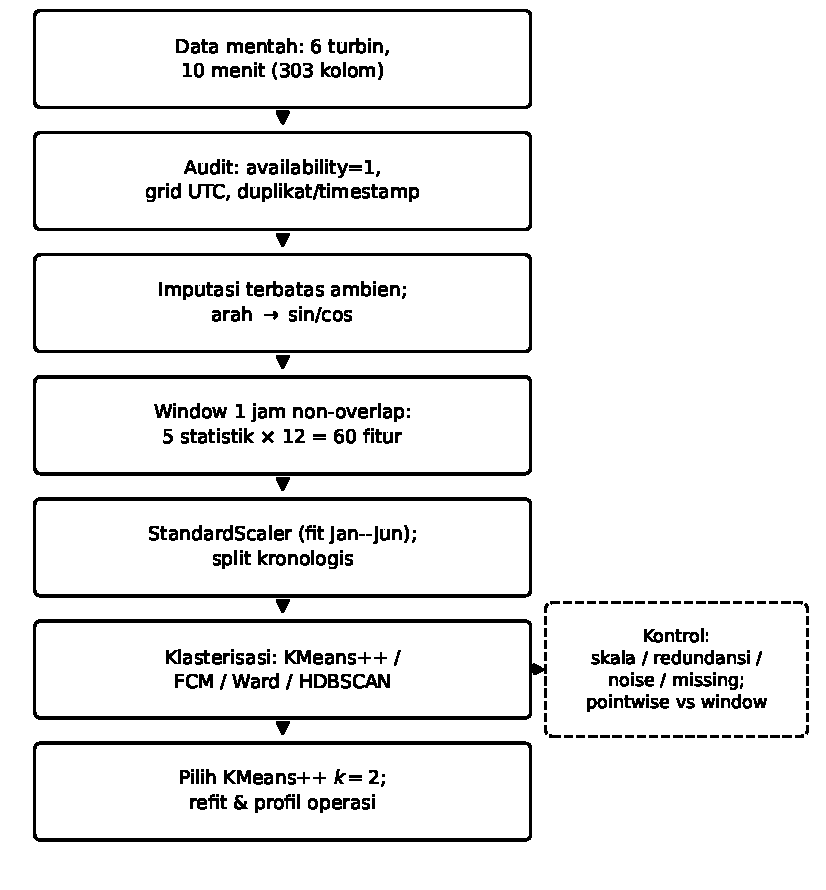
\includegraphics[width=0.64\columnwidth]{workflow.pdf}
\caption{Alur kerja preprocessing, klasterisasi, dan kontrol.}
\label{fig:workflow}
\end{figure}

\subsection{Data, audit, dan imputasi terbatas}
Enam turbin Senvion MM92 berdaya 2.050 kW/unit pada Kelmarsh versi 4 \cite{kelmarsh2025} dipetakan ke grid UTC tahun 2022. Availability=1 menyatakan observasi tersedia. Dari 302 kolom numerik dipilih 11 sinyal fisik yang dapat ditelusuri \cite{bonifati2022,bette2023,li2026}: angin/arah, daya aktif/reaktif, ambien, bearing generator depan, oli gearbox, rotor/generator, pitch blade A, dan frekuensi. Setpoint, waktu, identitas, flag, dan event hanya konteks. Fit menggunakan Januari--Juni; Juli--Desember untuk seleksi. Split kronologis adalah keputusan Kelmarsh, dengan pertimbangan missing-data dari \cite{ghaderi2023}, bukan final test independen.

\begin{table}[!t]
\centering
\caption{Rincian kumpulan data Kelmarsh 2022.}
\label{tab:dataset}
\footnotesize
\setlength{\tabcolsep}{4pt}
\begin{tabular}{lr}
\toprule
Aspek & Nilai \\
\midrule
Turbin (Senvion MM92) & 6 \\
Daya terpasang per turbin & 2.050 kW \\
Periode (UTC) & 2022, interval 10 menit \\
Slot terjadwal & 315.360 \\
Observasi tersedia & 314.018 \\
Kolom mentah (numerik) & 303 (302) \\
Sinyal fisik dipakai & 11 \\
Koordinat model & 12 \\
Fitur per window & 60 \\
Window final & 52.241 \\
\quad training (Jan--Jun) & 25.881 \\
\quad seleksi (Jul--Des) & 26.360 \\
Sel missing terisi & 19 (ambien) \\
\bottomrule
\end{tabular}
\end{table}

\textit{Pearson correlation} menilai hubungan linear untuk pasangan valid $\mathcal I$ \cite{bette2023,bonifati2022}:
\begin{equation}
r_{xy}=\frac{\sum_{i\in\mathcal I}(x_i-\bar x)(y_i-\bar y)}{\sqrt{\sum_{i\in\mathcal I}(x_i-\bar x)^2\sum_{i\in\mathcal I}(y_i-\bar y)^2}}.
\label{eq:pearson}
\end{equation}
$x_i,y_i$ ialah nilai dua sensor; $\bar x,\bar y$ mean pasangan valid. Spearman adalah korelasi peringkat; autokorelasi memasangkan sinyal dengan dirinya pada lag waktu nyata, tanpa menyambung gap.

\textit{Imputasi}, pengisian nilai hilang, mengadaptasi primitif \cite{bonifati2022,cai2025,ghaderi2023}. Benchmark tersimpan membandingkan penghapusan, median training, forward fill, linear, spline, KNN, dan mean turbin pada gap buatan 1/2/6/18 slot. Gate Kelmarsh menerima nRMSE $\leq0,10$ pada 1--2 slot, pengisian $\geq99\%$, dan tidak lebih buruk daripada median/forward fill. nRMSE adalah akar mean galat kuadrat ternormalisasi IQR training (simpangan baku bila IQR tidak positif; lalu 1 bila tidak valid). Median ialah nilai tengah; IQR ialah selisih kuartil ketiga dan pertama. Forward fill memakai nilai teramati terakhir; KNN (k-nearest neighbors) mengisi dari tetangga terdekat; spline memakai kurva polinomial tersambung. Hanya ambien lolos. Interpolasi linear menghubungkan dua batas dengan garis lurus:
\begin{equation}
\hat x(t)=x(t_L)+\frac{t-t_L}{t_R-t_L}[x(t_R)-x(t_L)],
\label{eq:linear}
\end{equation}
dengan $t_L,t_R$ batas teramati, $t_L<t<t_R$, $x$ ambien, dan $\hat x$ pengisian. Seluruh run hilang harus 1--2 slot (20 menit nilai hilang); run lebih panjang tidak diisi sebagian. Turbin/split tidak dilintasi. Dua slot hilang mempunyai batas teramati berselisih 30 menit; hanya 19 sel aktual diisi.

Penanganan ekstrem mengadaptasi \cite{ngophan2025,cai2025,li2026,belhadj2026}. IQR trimming (penghapusan di luar pagar kuartil), z-score trimming (penghapusan menurut jarak dari mean dalam unit std), winsorization (pembatasan ekstrem), DBSCAN (Density-Based Spatial Clustering of Applications with Noise, penapisan kepadatan), dan replacement regresi mempunyai benchmark tersimpan. Kebijakan akhir \textit{flag-only}: nilai tetap, tanpa trimming/replacement. Rentang fisik adalah heuristik audit, bukan batas pabrikan; arah di luar rentang tidak dikodekan. Flag bukan fitur atau label fault.

\subsection{Standardisasi, arah sirkular, dan window}
\textit{StandardScaler} mengadaptasi penyetaraan antar-satuan \cite{mazgula2024,bette2023,li2026}:
\begin{equation}
z_{ij}=\frac{x_{ij}-\mu_j}{\sigma_j},\qquad
\sigma_j^2=\frac{1}{N_T}\sum_{i\in\mathcal T}(x_{ij}-\mu_j)^2.
\label{eq:zscore}
\end{equation}
$j$ indeks fitur; $\mathcal T$ training, $N_T=|\mathcal T|$, dan $\mu_j$ mean training. Pembagi adalah $N_T$ (ddof=0); skala nol diganti 1. Median training mengisi nilai kosong untuk fit scaler benchmark titik, tanpa menjadikannya pengukuran final. Global Standard dipilih terhadap Min--Max (minimum/rentang) dan Robust (median/IQR); parameter dibekukan untuk seleksi.

\textit{Circular encoding} mengadaptasi representasi arah \cite{cai2025,lang2026}, dengan sudut $\theta(t)$ dalam derajat:
\begin{equation}
d_{\sin}(t)=\sin\frac{\pi\theta(t)}{180},\quad d_{\cos}(t)=\cos\frac{\pi\theta(t)}{180}.
\label{eq:circular}
\end{equation}
$d_{\sin},d_{\cos}$ ialah koordinat arah tanpa satuan; sudut melingkar menyamakan $0^\circ$ dan $360^\circ$. Sepuluh skalar dan pasangan arah menghasilkan 12 koordinat. Sin/cos titik memakai skala unit sama; untuk setiap statistik window, skala pasangan diganti akar rata-rata kuadrat kedua skala training, dengan mean tetap per koordinat.

\textit{Window non-overlap} adalah interval tanpa tumpang tindih \cite{martipuig2024,bonifati2022,lang2026,bette2023}. Aturan benchmark memilih durasi terpendek dengan retensi seleksi $\geq80\%$, lalu kelengkapan paling ketat; terpilih satu jam, $L=6$ slot lengkap. Untuk nilai berurutan $v_{w\ell j}$ dalam window $w$, lima statistik mengikuti representasi bernama \cite{bonifati2022}:
\begin{align}
\bar v_{wj}&=\frac{1}{L}\sum_{\ell=1}^{L}v_{w\ell j},\quad
s_{wj}=\sqrt{\frac{\sum_{\ell=1}^{L}(v_{w\ell j}-\bar v_{wj})^2}{L-1}},\label{eq:windowstats}\\
v^{\min}_{wj}&=\min_\ell v_{w\ell j},\quad v^{\max}_{wj}=\max_\ell v_{w\ell j},\nonumber\\
\Delta v_{wj}&=v_{wLj}-v_{w1j}.\label{eq:endpoint}
\end{align}
$\ell=1,\ldots,L$ adalah urutan slot; $\bar v,s,v^{\min},v^{\max},\Delta v$ ialah mean, std sampel (ddof=1), minimum, maksimum, dan perubahan endpoint (selisih, bukan slope/jam). Statistik dibentuk dari nilai fisik setelah interpolasi diterima dan pasangan arah, bukan kolom scalar-scaled titik. Enam puluh statistik distandardisasi tersendiri pada window training, dengan shared scale sin/cos per statistik. Median/flag imputasi koordinat disimpan sebagai pengaman. Urutan fitur, scaler, dan SHA-256 input tetap untuk semua kandidat. PCA (proyeksi), DCT (kompresi frekuensi), tsfresh (ekstraksi otomatis), PFA (seleksi fitur asli), serta smoothing/derivative hanya diagnostik alternatif, tidak pada input utama \cite{bonifati2022,martipuig2024}.

\subsection{Kandidat klasterisasi yang telah dijalankan}
Dalam pemodelan, $\mathcal T$ dan $N_T$ merujuk window training. Tuliskan $\mathbf x_i\in\mathbb R^{60}$ sebagai vektor window terstandar; $C_j$ klaster, $k$ jumlah diminta, dan $\mathbf c_j$ centroid.
\textit{K-Means} meminimalkan kuadrat jarak Euclidean:
\begin{equation}
J_{\mathrm{KM}}=\sum_{j=1}^{k}\sum_{i\in C_j}\|\mathbf x_i-\mathbf c_j\|_2^2.
\label{eq:kmeans}
\end{equation}
$\mathbf c_j$ mean anggota $C_j$ dan $\|\cdot\|_2$ norma Euclidean. Baseline berbasis fitur mengikuti \cite{bonifati2022,ngophan2025}; seeding K-Means++ berbobot jarak kuadrat memakai varian greedy scikit-learn. Konfigurasi aktual $k=2$--10, Lloyd, 20 inisialisasi, 500 iterasi maksimum, toleransi relatif perpindahan pusat $10^{-4}$, seed 2022; lima seed 2022--2026 mengaudit stabilitas tiap $k$.

\textit{Fuzzy C-Means} (FCM) memberi keanggotaan beberapa pusat:
\begin{equation}
J_m=\sum_{i=1}^{N_T}\sum_{j=1}^{k}u_{ij}^{m}\|\mathbf x_i-\mathbf c_j\|_2^2.
\label{eq:fcm}
\end{equation}
$u_{ij}\in[0,1]$, $\sum_j u_{ij}=1$, dan fuzzifier $m>1$ mengatur kekaburan. FCM standar menguji soft assignment \cite{cai2025}, tanpa optimizer/forecasting mereka. Scikit-fuzzy memakai $m=2$, $k=2$--10, lima seed, 500 iterasi maksimum, serta penghentian $\|U^{(r+1)}-U^{(r)}\|_F<10^{-5}$ ($U$ matriks keanggotaan, $r$ iterasi, norma Frobenius). Inisialisasi konvergen dipilih berdasarkan objektif training; pusat tetap memberi keanggotaan seleksi dan hard label $\arg\max_j u_{ij}$. FPC, jumlah kuadrat keanggotaan dibagi banyak objek, mendekati $1/k$ bila seragam; entropi ternormalisasi mendekati 1. Ambiguitas memakai $\max_j u_{ij}<0,60$.

\textit{HDBSCAN}, hierarki kepadatan dengan label noise \cite{ngophan2025}, menguji enam kombinasi minimum klaster $100/300/800$ dan minimum sampel $10/30$ pada semua training. Pustaka hdbscan 0.8.44 memakai Euclidean, \texttt{prims\_kdtree}, excess-of-mass, dan prediction data. Jumlah kelompok tidak dikendalikan $k$. Approximate prediction seleksi memakai struktur training tetap, tanpa kelompok baru; noise $-1$ disimpan.

\textit{Agglomerative Ward} menggabungkan $A,B$ dengan kenaikan kuadrat intraklaster terkecil:
\begin{equation}
\Delta J(A,B)=\frac{|A||B|}{|A|+|B|}\|\mathbf c_A-\mathbf c_B\|_2^2.
\label{eq:ward}
\end{equation}
$|A|,|B|$ jumlah anggota, $\mathbf c_A,\mathbf c_B$ centroid. Keluarga hierarkis dimotivasi \cite{martipuig2024}, tetapi linkage adalah keputusan Kelmarsh. $k=2$--10 memakai 4.000 training deterministik karena memori; K-Means pembanding di-fit pada sampel sama. Tidak ada prediksi seleksi Ward. GMM tidak dijalankan karena justifikasi empiris tambahan belum ditetapkan.

\subsection{Rancangan kontrol dan representasi}
Untuk memisahkan pengaruh pilihan preprocessing dari algoritma, dilakukan kontrol satu faktor: satu keputusan diubah sementara sisanya tetap pada konfigurasi referensi (StandardScaler, 60 statistik, tanpa pembatasan ekstrem, missing ambien-terbatas) dengan K-Means++ $k=2$, seed, dan fitur yang sama. Setiap varian dinilai dengan Silhouette, DBI, dan CHI, ditambah \textit{Adjusted Rand Index} (ARI), yaitu kesesuaian partisi terkoreksi peluang; ARI mendekati 1 berarti struktur hampir tidak berubah dan mendekati 0 berarti partisi berbeda. Ukuran klaster terkecil, stabilitas seed, dan persistence juga dicatat agar skor tinggi akibat kelompok mungil dapat dikenali.

Faktor skala membandingkan tanpa scaling, StandardScaler (referensi), \textit{RobustScaler} (median dan IQR, lebih tahan pencilan), \textit{Min--Max} (pemetaan linear ke $[0,1]$), dan standardisasi per-turbin; primitif penyetaraan skala mengikuti \cite{mazgula2024,li2026,bette2023}, sedangkan pemilihan dan penolakan varian merupakan keputusan benchmark Kelmarsh. Faktor redundansi membandingkan 60 statistik (referensi) dengan hanya 12 mean koordinat, pembuangan keluarga generator, representasi level-tambah-dinamika, dan pembuangan keluarga frekuensi; motivasi menghapus fitur derived dan redundan mengikuti \cite{bonifati2022,li2026,bette2023}. Faktor ekstrem membandingkan tanpa pembatasan dengan \textit{winsorization}, yaitu pembatasan nilai ke persentil, pada $1$--$99$ dan $5$--$95$ \cite{cai2025,belhadj2026}. Faktor missing membandingkan kebijakan ambien-terbatas (referensi), pembuangan baris (\textit{listwise}), median training, dan forward fill \cite{bonifati2022,cai2025,ghaderi2023}.

Kontrol representasi temporal membandingkan klasterisasi observasi 10 menit individual (pointwise) dengan window satu jam pada 12 sinyal, scaler, split, dan algoritma yang sama, sehingga perbedaan bersumber dari agregasi temporal; gagasan window versus observasi tunggal dimotivasi \cite{martipuig2024,draayer2026,lang2026}. Selain indeks internal, diukur koherensi temporal berupa panjang run (rata-rata dan median durasi label bertahan, dalam jam), laju pergantian label per jam, dan ARI antara label window dan label pointwise setelah label window dipetakan ke enam observasi anggotanya.

\subsection{Validitas, kontinuitas, dan pemilihan}
Pada populasi evaluasi $E$, \textit{Silhouette} adalah mean
\begin{equation}
s_i=\frac{b_i-a_i}{\max(a_i,b_i)},
\label{eq:silhouette}
\end{equation}
$a_i$ mean jarak ke anggota klaster sendiri di $E$ dan $b_i$ mean jarak minimum ke klaster lain; singleton diberi nol. Untuk K-Means/FCM, $E$ adalah 3.000 seleksi deterministik; jarak dihitung di dalam sampel, bukan semua 26.360. HDBSCAN dan K-Means matched memakai irisan sampel dengan non-noise yang sama; Ward memakai 3.000 dari sampel training bersama.

\textit{Davies--Bouldin Index} mengukur rasio sebaran/pemisahan:
\begin{equation}
\mathrm{DBI}=\frac{1}{K}\sum_{j=1}^{K}\max_{h\ne j}\frac{S_j+S_h}{\|\mathbf c_j-\mathbf c_h\|_2}.
\label{eq:dbi}
\end{equation}
$K$ jumlah label terisi; $S_j$ mean jarak objek ke centroid klaster $j$. \textit{Calinski--Harabasz Index} membandingkan dispersi:
\begin{equation}
\mathrm{CHI}=\frac{\sum_j n_j\|\mathbf c_j-\bar{\mathbf x}\|_2^2/(K-1)}{\sum_j\sum_{i\in C_j}\|\mathbf x_i-\mathbf c_j\|_2^2/(N-K)}.
\label{eq:chi}
\end{equation}
$n_j=|C_j|$, $N$ ukuran populasi, dan $\bar{\mathbf x}$ mean seluruh populasi. DBI/CHI memakai seleksi penuh, non-noise matched, atau 4.000 training sesuai eksperimen. Silhouette/CHI lebih tinggi dan DBI lebih rendah dibaca pada populasi sebanding; indeks tidak dipakai bila label terisi tidak cukup.

\textit{Adjusted Rand Index} (ARI) menilai kesesuaian partisi terkoreksi peluang; Normalized Mutual Information (NMI) menilai asosiasi label dengan identitas/flag, bukan akurasi operasi. Temporal persistence, diagnostik kontinuitas yang dimotivasi \cite{lang2026}, adalah
\begin{equation}
P=\frac{1}{|\mathcal A|}\sum_{(i,h)\in\mathcal A}\mathbf1[g(i)=g(h)].
\label{eq:persistence}
\end{equation}
$g(i)$ label; $\mathbf1$ indikator; $\mathcal A$ pasangan pada turbin dan split sama, tepat satu jam, tanpa melintasi gap. HDBSCAN all-label dan assigned-only mempunyai penyebut berbeda. Pemilihan mempertimbangkan indeks \cite{ngophan2025,li2026}, kelompok kecil (peringatan $<1\%$), seed, kontinuitas, profil, dan cakupan. Refit seluruh tahun yang sudah tersedia dilakukan setelah pemeriksaan kandidat, dengan scaler training tetap; profil refit dipisahkan dari skor seleksi.

